% Provenance (never printed): see sources/outline_sources.md (Year 2: Hadean, Archean and
% Proterozoic; early crust and greenstone belts; the oxygenation of the atmosphere; snowball
% Earth). Eons and eras from the ICS chart; greenstone belts, TTG and cratons after Cawood and
% others (2018) and Smithies and others (2019); komatiite liquidus after Sossi and O'Neill (2016),
% Pierru and others (2022) and Asimow (2022); the Archean air and the GOE after Catling and Zahnle
% (2020) and Luo and others (2016); the boring billion after Lyons and others (2021); snowball
% Earth after Hoffman and others (2017). The energy-balance model, the komatiite line and the CO2
% build-up from figdata/bachelor-2/precambrian.py; exercise and problem values in the Book 4
% scratch calculator calc/ch18.py.
\chapter{前寒武纪地球}\label{ch:b2:precambrian-earth}

最早的贝壳状化石出现在约 5.4 亿年前的岩层中。此前的一切，
即自地球诞生（距今 \qty{4567}{Ma}）起的全部历史，属于前寒武纪，占地球历史的八分之七。
在此期间，地球形成了大陆的核心，大气中充满了氧气，
并且至少两次从两极到赤道全面冰封，冰盖一直延伸到
热带的海边。本章从留存下来的岩石中解读这四十亿年的历史，
并用数字回答其中三个谜题：最古老的熔岩为何如此灼热，冰封的
行星如何解冻，以及年轻的地球在暗淡的太阳下如何保持温暖。
% ledger: ics:base.Hadean, ics:base.Phanerozoic, hoffman17:cryochrons

\begin{recall}
\textbf{来自中学阶段各册}：地球年龄；地质年代表上的宙；
年轻太阳的光度定律与\omterm{def:b2:precambrian-earth:faint-sun}{黯淡太阳悖论}；原始大气；
叠层石、\omterm{def:b2:precambrian-earth:bif}{条带状铁建造}、\omterm{def:b2:precambrian-earth:goe}{大氧化事件}和红层；\omterm{def:b2:precambrian-earth:craton}{克拉通}；
过去的放射性生热。\textbf{来自本科一年级分册}：锆石及其 U--Pb 年龄，
封闭温度；四种同位素的放射性生热率；向外长波
辐射与全球平均日射量 $S_0/4$；年代地层单位。
\textbf{来自前面各章}：\omterm{def:b2:mantle-melting:tp}{地幔位温}与绝热线
（\cref{ch:b2:mantle-melting}）；橄榄石的液相线与\omterm{def:b2:magmatic-differentiation:crystallisation}{分离结晶}
（\cref{ch:b2:magmatic-differentiation}）；花岗岩类型（\cref{ch:b2:crustal-melting}）；
\omterm{def:b2:wilson-cycle:supercontinent}{超大陆}（\cref{ch:b2:wilson-cycle}）。氧化与还原属于化学分册，
最早的真核生物与光合作用则属于生物分册。
\end{recall}

\section{化石出现之前的三个宙}\label{sec:b2:precambrian-earth:eons}

\begin{definition}[冥古宙、太古宙、元古宙]\label{def:b2:precambrian-earth:eons}
显生宙之前的时间划分为三个宙。其中\emph{冥古宙}\index{冥古宙}
始于地球形成之时（距今 \qty{4567}{Ma}），止于 $4031 \pm \qty{3}{Ma}$；
\emph{太古宙}\index{太古宙}，介于 $4031$ 至 \qty{2500}{Ma} 之间；
\emph{元古宙}\index{元古宙}介于 2500 至 \qty{538.8}{Ma} 之间，即寒武纪底界。
三者合称前寒武纪。
\end{definition}
% ledger: ics:base.Hadean, ics:base.Archean, ics:base.Proterozoic, ics:base.Phanerozoic

\omterm{def:b2:precambrian-earth:eons}{太古宙}分为四个代：始太古代（4031 至 \qty{3600}{Ma}）、古太古代（3600
至 3200）、中太古代（3200 至 2800）和新太古代（2800 至 2500）；\omterm{def:b2:precambrian-earth:eons}{元古宙}分为三个代，
即古元古代（2500 至 \qty{1600}{Ma}）、中元古代（1600 至 1000）和
新元古代（1000 至 538.8）。下文涉及新元古代的两个纪：成冰纪，720 至
\qty{635}{Ma}，以及埃迪卡拉纪，635 至 \qty{538.8}{Ma}。
% ledger: ics4:archean-eras, ics4:proterozoic-eras

\begin{omfigure}
\centering
% ledger: ics:base.Hadean, ics:base.Archean, ics:base.Proterozoic, ics:base.Phanerozoic, ics4:archean-eras, ics4:proterozoic-eras, wilde01:4404, bowring99:acasta, cz20:impacts, allwood06:spc, cawood18:transition, gumsley17:goe, luo16:goe, hoffman17:earlier, earle:bif, lyons21:boring, hoffman17:ages, asimow22:komatiite
\begin{tikzpicture}[x=-3.4cm, y=1cm, font=\scriptsize]
% eons
\fill[icsHadean] (4.567,0) rectangle (4.031,0.5);
\fill[icsArchean] (4.031,0) rectangle (2.5,0.5);
\fill[icsProterozoic] (2.5,0) rectangle (0.5388,0.5);
\fill[icsPhanerozoic] (0.5388,0) rectangle (0,0.5);
\node[text=white] at (4.299,0.25) {冥古宙};
\node[text=white] at (3.27,0.25) {太古宙};
\node[text=white] at (1.52,0.25) {元古宙};
\node at (0.27,0.25) {显生宙};
% eras
\foreach \a/\b/\c in {4.031/3.6/35, 3.6/3.2/55, 3.2/2.8/35, 2.8/2.5/55}
  \fill[icsArchean!\c] (\a,-0.45) rectangle (\b,0);
\foreach \a/\b/\c in {2.5/1.6/35, 1.6/1.0/55, 1.0/0.5388/35}
  \fill[icsProterozoic!\c] (\a,-0.45) rectangle (\b,0);
\foreach \x/\l in {3.8155/始, 3.4/古, 3.0/中, 2.65/新, 2.05/古, 1.3/中, 0.769/新}
  \node at (\x,-0.225) {\l};
% axis
\draw (4.6,-0.6) -- (0,-0.6);
\foreach \t in {0,0.5,...,4.5} {
  \draw (\t,-0.6) -- (\t,-0.7);
  \node[anchor=north] at (\t,-0.7) {\pgfmathprintnumber[fixed, precision=1]{\t}};
}
\node[anchor=north, font=\small] at (2.3,-1.05) {距今时间（十亿年）};
% row A
\fill[omDef] (4.404,0.85) circle (2pt);
\node[anchor=west, text=omDef] at (4.404,0.85) {最古老锆石};
\fill[omMeth] (3.43,0.85) circle (2pt);
\node[anchor=west, text=omMeth] at (3.43,0.85) {最早的叠层石};
\draw[red!60!black, line width=3pt] (2.4,0.85) -- (1.8,0.85);
\node[anchor=west, text=red!60!black] at (1.8,0.85) {条带状铁建造};
% row B
\fill[omDef] (4.03,1.5) circle (2pt);
\node[anchor=west, text=omDef] at (4.03,1.5) {最古老岩石};
\draw[black!70, line width=3pt] (3.2,1.5) -- (2.5,1.5);
\node[anchor=south, text=black!80] at (2.85,1.6) {构造风格转变};
\draw[omProp, line width=3pt] (1.8,1.5) -- (0.8,1.5);
\node[anchor=south, text=omProp] at (1.3,1.6) {“乏味的十亿年”};
% row C
\draw[black!60, line width=2pt, densely dashed] (4.2,2.25) -- (3.5,2.25);
\node[anchor=south, text=black!70] at (3.85,2.35) {晚期重轰炸？（有争议）};
\draw[omThm, line width=3pt] (2.43,2.25) -- (2.06,2.25);
\node[anchor=west, text=omThm] at (2.06,2.25) {大氧化事件};
% row D
\fill[blue!60!black] (2.4,3.0) circle (2pt);
\node[anchor=east, text=blue!60!black] at (2.4,3.0) {首次雪球地球};
\fill[omThm] (0.8,3.0) circle (2pt);
\node[anchor=east, text=omThm] at (0.8,3.0) {第二次氧气上升};
% row E
\fill[orange!80!black] (1.9,3.7) circle (2pt);
\node[anchor=east, text=orange!80!black] at (1.9,3.7) {最后的普通科马提岩};
\draw[blue!60!black, line width=3pt] (0.717,3.7) -- (0.635,3.7);
\node[anchor=east, text=blue!60!black] at (0.717,3.7) {成冰纪雪球地球};
% row F
\fill[omMeth] (0.57,4.4) circle (2pt);
\node[anchor=east, text=omMeth] at (0.57,4.4) {最早的大型化石（埃迪卡拉纪）};
\end{tikzpicture}
\par\smallskip{\small 前寒武纪一览。宙，以及以较浅色调表示的代
（始、古、中、新太古代；古、中、新元古代）为
国际年代地层表所列；事件按正文所给年龄标注。
“最后的普通\omterm{def:b2:precambrian-earth:greenstone}{科马提岩}”指未贫铝者；较年轻、较少见的类型也存在。}
\end{omfigure}

\subsection*{冥古宙：只有矿物，没有岩石}

\omterm{def:b2:precambrian-earth:eons}{冥古宙}没有岩石留存下来，只有矿物。最古老的是一颗锆石，产自西澳大利亚的
杰克山，年龄为 $4404 \pm \qty{8}{Ma}$，它被冲刷出更老的岩石，约 30 亿年前沉积于砾岩中。
该锆石及其邻近矿物的成分被发现者解读为证据，
表明大陆型地壳与
液态水在 \qty{4.4}{Ga} 前（即地球形成约 1.6 亿年后）已经存在。
定年最古老的岩石是加拿大西北部的阿卡斯塔片麻岩，年龄为 4.00 至
\qty{4.03}{Ga}，接近\omterm{def:b2:precambrian-earth:eons}{太古宙}的底界。
% ledger: wilde01:4404, wilde01:zircon, uw14:jack-hills, bowring99:acasta

年轻的地球曾遭受大天体的撞击，正如\cref{ch:b2:planet-formation-meteorites}
所述。能使整个海洋汽化的最后一次大撞击
估计发生于约 \qty{4.3}{Ga} 前。此后提出的“晚期重轰炸”，
是一阵集中的撞击，发生于约 4.2--4.0 至 \qty{3.5}{Ga} 之间，据月球岩石和\omterm{def:b2:planet-formation-meteorites:fall-find}{陨石}冲击痕迹的
年龄推断而来，已被提出。许多人质疑它是否确为一个独立事件，
无论哪种情况，它大概都不会使地球失去生命。
% ledger: cz20:impacts

\section{太古宙地壳}\label{sec:b2:precambrian-earth:archean}

\subsection*{绿岩带与科马提岩}

保存至今的\omterm{def:b2:precambrian-earth:eons}{太古宙}地壳由两类并列的\omterm{def:b2:wilson-cycle:terrane}{地体}构成：大片
灰色富钠花岗质片麻岩，以及较窄的蚀变火山岩与沉积岩带。

\begin{definition}[绿岩带；科马提岩]\label{def:b2:precambrian-earth:greenstone}
称\emph{绿岩带}\index{绿岩带}为由镁铁质和超镁铁质火山岩组成的岩带，
其中夹有沉积物，经低级变质（绿色来源于绿泥石、阳起石和
绿帘石），位于\omterm{def:b2:precambrian-earth:eons}{太古宙}及部分\omterm{def:b2:precambrian-earth:eons}{元古宙}的花岗岩类岩体之间。
称\emph{科马提岩}\index{科马提岩}为超镁铁质熔岩，MgO 含量远高于玄武岩，
以液态喷出；其中的橄榄石通常长成细长的晶片，
形成\emph{鬣刺结构}，因为熔岩流顶部冷却迅速。
\end{definition}
% ledger: cawood18:dome-keel, so16:liquidus, pierru22:komatiite

\begin{omfigure}
\centering
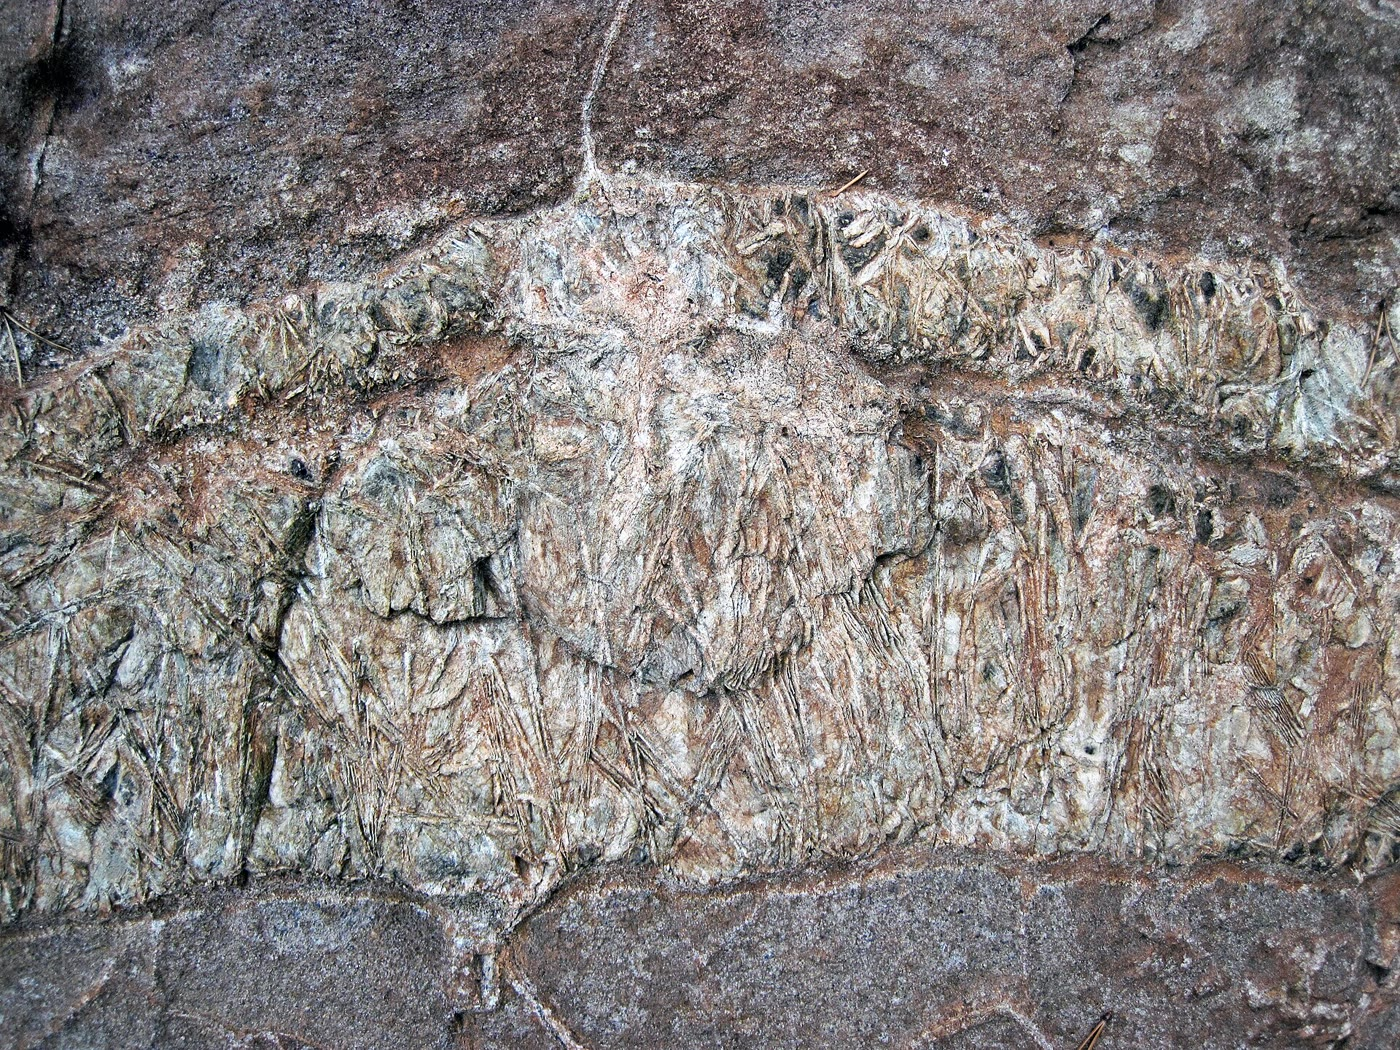
\includegraphics[width=0.66\linewidth]{images/book4/b2-18-spinifex-komatiite.jpg}
\par\smallskip{\small \omterm{def:b2:precambrian-earth:greenstone}{科马提岩}熔岩流中的鬣刺结构，位于安大略省派克山，属于
新太古代\omterm{def:b2:precambrian-earth:greenstone}{绿岩带}的一部分，年龄约 27.1 亿年：现已蚀变的橄榄石晶片
横跨熔岩流冷却的顶部生长。照片：James St.~John, CC~BY~2.0（维基
共享资源）。}
\end{omfigure}

\omterm{def:b2:precambrian-earth:greenstone}{科马提岩}的 MgO 含量可达 \qty{34}{\percent}，而今日洋脊的原生
玄武岩仅为 10 至 \qty{13}{\percent}。\omterm{def:b2:precambrian-earth:greenstone}{科马提岩}几乎只见于古老的地球，其中贫铝类型
只见于老于 \qty{2.8}{Ga} 的岩石中，未贫铝类型则延续至约
\qty{1.9}{Ga}，而仅有少量富铝类型，年龄可小至 \qty{90}{Ma}。熔体
如此富镁，温度很高；与
\cref{ch:b2:magmatic-differentiation}中的玄武岩类似，最先从中结晶出的矿物是橄榄石，
其在熔体中的占比决定了温度。
% ledger: pierru22:komatiite, asimow22:komatiite

\begin{proposition}[科马提岩温度计]\label{prop:b2:precambrian-earth:liquidus}
对于在大气压强下与橄榄石处于平衡的熔体，其液相线温度
近似线性地随熔体的 MgO 含量升高。经过两次实验 $(m_1, T_1)$ 与
$(m_2, T_2)$ 确定的直线为：
\[
  T_{\text{liq}}(m) = T_1 + s\,(m - m_1), \qquad s = \frac{T_1 - T_2}{m_1 - m_2} .
\]
两种\omterm{def:b2:precambrian-earth:greenstone}{科马提岩}的熔融实验：MgO 为 $\qty{32.2}{\percent}$ 时，温度 \qty{1616}{\celsius}；
MgO 为 $\qty{23}{\percent}$ 时，温度 \qty{1450}{\celsius}。由此得 $s = \qty{18.0}{\celsius}$，
即每百分之一 MgO。
\end{proposition}
% ledger: so16:liquidus, helz98:glass-thermometer

\begin{proof}
橄榄石是镁橄榄石与铁橄榄石的固溶体，其镁含量远高于
它所生长的熔体。熔体冷却时，橄榄石从中夺取镁，使熔体恰好
被橄榄石饱和的温度随 MgO 含量降低而下降。实验表明，
在某一类熔体的成分范围内，这一下降近似为线性，因此经过
两次实验的直线在二者之间内插：$s = (1616 - 1450)/(32.2 - 23) = 166/9.2 = 18.04$。
\end{proof}

该系数并非\omterm{def:b2:precambrian-earth:greenstone}{科马提岩}所独有。取自基拉韦厄火山熔岩的淬火玻璃，
以同样方式标定，MgO 含量变化 \qty{0.15}{\percent} 时，温度变化 \qty{3}{\celsius}，
合每百分之一 MgO \qty{20}{\celsius}。将\omterm{def:b2:precambrian-earth:greenstone}{科马提岩}的直线外推至
原生洋脊玄武岩（MgO 为 \qty{12}{\percent}），由此可得其液相线温度，精度在几十摄氏度以内：$1616 -
18.0\times20.2 \approx \qty{1252}{\celsius}$。因此，最热的\omterm{def:b2:precambrian-earth:greenstone}{科马提岩}熔体
比供给今日洋脊的熔体高约 \qty{360}{\celsius}，下图
给出了这条直线。
% ledger: helz98:glass-thermometer, so16:liquidus, pierru22:komatiite
% values: slope 18.043, T_morb12 1251.5, dT_kom_morb 364.5 (precambrian.py)

\begin{omfigure}
\centering
\begin{tikzpicture}
\begin{axis}[omrecord, width=0.72\linewidth, height=6cm, xmin=8, xmax=35, ymin=1150, ymax=1700,
  xlabel={熔体中 MgO 含量（\unit{\percent}，按质量）}, ylabel={1 atm 下液相线温度（\unit{\celsius}）},
  xtick pos=bottom, ytick pos=left, clip=false,
  y tick label style={/pgf/number format/1000 sep={}}]
% computed in figdata/bachelor-2/precambrian.py part kom; ledger: so16:liquidus, pierru22:komatiite
\fill[omProp!15] (axis cs:10,1150) rectangle (axis cs:13,1700);
\addplot[black, line width=1.1pt] table[x=MgO, y=T] {figdata/out/bachelor-2-precambrian-kom.dat};
\addplot[only marks, mark=*, mark size=2.4pt, omThm] coordinates {(32.2,1616) (23,1450)};
\node[anchor=north west, font=\scriptsize, text=omThm] at (axis cs:32.2,1612) {巴伯顿};
\node[anchor=north west, font=\scriptsize, text=omThm] at (axis cs:23,1446) {孟罗};
\node[anchor=south, font=\scriptsize, text=omProp, align=center] at (axis cs:11.5,1560)
  {原生 \\洋脊玄武岩};
\draw[densely dashed] (axis cs:12,1150) -- (axis cs:12,1251.5) -- (axis cs:8,1251.5);
\draw[densely dashed] (axis cs:32.2,1150) -- (axis cs:32.2,1616);
\draw[<->, omDef, thick] (axis cs:27,1251.5) -- (axis cs:27,1616);
\draw[densely dotted] (axis cs:12,1251.5) -- (axis cs:27,1251.5);
\draw[densely dotted] (axis cs:27,1616) -- (axis cs:32.2,1616);
\node[anchor=east, font=\scriptsize, text=omDef] at (axis cs:26.7,1330) {约 \qty{360}{\celsius}};
\end{axis}
\end{tikzpicture}
\par\smallskip{\small \omterm{def:b2:precambrian-earth:greenstone}{科马提岩}温度计：过两种\omterm{def:b2:precambrian-earth:greenstone}{科马提岩}（圆点）测得液相线温度的直线，
外推至今日洋脊原生玄武岩的 10 至 \qty{13}{\percent} MgO
含量范围（色带）。外推依据是玄武质熔体的斜率相近。}
\end{omfigure}

熔岩温度更高，并不意味着地幔的温度也高出同样的幅度。\omterm{def:b2:precambrian-earth:greenstone}{科马提岩}很可能是以地幔柱的形式
上升的，正如今日最热的玄武岩在夏威夷所表现的那样：那里的位温最多可高出约 \qty{200}{\celsius}，
而周围地幔的温度为 $1350 \pm \qty{50}{\celsius}$。
它们由较大程度的\omterm{def:b2:mantle-melting:melting}{部分熔融}形成，且形成于更大的深度。一般认为，它们
形成于比今天高 200 至 \qty{300}{K} 的地幔之中；另一种观点认为，\omterm{def:b2:precambrian-earth:greenstone}{科马提岩}是
富水\omterm{def:b2:magma-emplacement:magma}{岩浆}，形成温度并不比周围地幔高出多少。
无论哪种观点，\omterm{def:b2:precambrian-earth:eons}{太古宙}地幔都更热。高中分册
给出了一个理由：30 亿年前，四种放射性同位素释放的热量
是今日的两倍以上（见\cref{exo:b2:precambrian-earth:2}）。
% ledger: asimow22:komatiite, pierru22:komatiite, so16:liquidus

\subsection*{TTG 与穹隆–龙骨构造}

\omterm{def:b2:precambrian-earth:greenstone}{绿岩带}之间的灰色片麻岩，并不是
在\cref{ch:b2:crustal-melting}中所描述的那类花岗岩。

\begin{definition}[英云闪长岩–奥长花岗岩–花岗闪长岩组合]\label{def:b2:precambrian-earth:ttg}
称\emph{英云闪长岩–奥长花岗岩–花岗闪长岩组合}\index{英云闪长岩–奥长花岗岩–花岗闪长岩组合}（TTG）为
一类富钠贫钾的花岗质岩石族，包括英云闪长岩、
奥长花岗岩（镁铁质矿物较少的英云闪长岩）和花岗闪长岩，构成了\omterm{def:b2:precambrian-earth:eons}{太古宙}大陆地壳的大部分。
其中大多数由含水玄武质
地壳\omterm{def:b2:mantle-melting:melting}{部分熔融}而成。
\end{definition}
% ledger: smithies19:ttg, cawood18:ttg

今日大陆地壳的大部分体积在\omterm{def:b2:precambrian-earth:eons}{太古宙}末已经形成，主要为
TTG。部分 TTG 的\omterm{def:b2:elements-in-the-earth:trace}{微量元素}特征长期被解读为在超过
\qty{50}{km} 深度下熔融的结果，这一压强在较年轻的大陆地壳中达不到，这些解读
与关于板块构造何时开始的争论有关；2019 年的一项研究认为，这些特征
实际上来自地幔熔体，而常见的 TTG 形成于
不超过今日普通大陆地壳的 \qty{40}{km} 深度。\omterm{def:b2:precambrian-earth:eons}{太古宙}晚期，
约 3.0 至 \qty{2.5}{Ga} 之间，多数\omterm{def:b2:precambrian-earth:craton}{克拉通}的花岗质岩由 TTG 转变为
富钾花岗岩，这标志着更厚的地壳再次发生了熔融。
% ledger: smithies19:ttg, cawood18:ttg

在澳大利亚东部的皮尔巴拉、津巴布韦和印度南部，这两类\omterm{def:b2:wilson-cycle:terrane}{地体}在地图上勾勒出
一幅醒目的图案：圆形的花岗质穹隆被向斜状的绿岩龙骨环绕，龙骨中的岩层向外倾斜，背离穹隆。
一般认为，穹隆是以\omterm{def:b2:magma-emplacement:ascent}{底辟}的形式上升的：较轻的花岗质地壳穿过厚而致密的
熔岩堆，这些熔岩曾在穹隆之间下沉。在皮尔巴拉，这种穹隆化持续了数亿
年之久，大约在 \qty{3.1}{Ga} 前停止，此后这些构造
变为线状，与较年轻\omterm{def:b2:alpine-orogen:orogen}{造山带}中的构造相似。
% ledger: cawood18:dome-keel

\begin{omfigure}
\centering
\begin{tikzpicture}[x=0.95cm, y=0.95cm, font=\scriptsize]
% schematic, after the description in cawood18:dome-keel
\fill[lith basalt] (0,0) rectangle (12,7);
\draw (0,0) rectangle (12,7);
\foreach \cx/\cy/\rx/\ry in {2.4/4.7/1.7/1.4, 7.2/5.0/2.0/1.4, 4.6/1.6/1.9/1.1, 10.0/2.0/1.4/1.3}
  \filldraw[lith granite, draw=black, thick] (\cx,\cy) ellipse ({\rx} and {\ry});
% strike and dip in the greenstone, each dipping away from the nearest dome
% (positions and strikes from the outward normals of the ellipses, computed by hand)
\foreach \px/\py/\st in {3.9/5.99/309, 0.9/5.99/231, 0.9/3.41/129, 2.4/2.88/90, 4.52/4.7/0,
    9.62/5.0/0, 8.91/6.29/305, 5.49/6.29/235, 8.91/3.71/55, 5.49/3.71/125,
    6.92/1.6/0, 4.6/3.12/270, 2.28/1.6/180, 6.24/0.53/60,
    10.0/3.72/270, 11.29/0.78/47, 8.18/2.0/180, 11.29/3.22/313}
  \pic at (\px,\py) {strikedip={\st}{}};
\node[fill=white, inner sep=1.5pt] at (2.4,4.7) {TTG 穹隆};
\node[fill=white, inner sep=1.5pt] at (7.2,5.0) {TTG 穹隆};
\node[fill=white, inner sep=1.5pt] at (4.6,1.6) {TTG 穹隆};
\node[fill=white, inner sep=1.5pt] at (10.0,2.0) {TTG 穹隆};
\node[fill=white, inner sep=1.5pt, align=center] at (7.45,2.75) {绿岩 \\龙骨};
\node[fill=white, inner sep=1.5pt, align=center] at (1.0,0.9) {绿岩};
\pic at (11.4,5.6) {northarrow};
% section below
\begin{scope}[yshift=-3.3cm]
\fill[lith basalt] (0,0) -- (12,0) -- (12,2.2) -- (0,2.2) -- cycle;
\filldraw[lith granite, draw=black, thick] (0.6,0) .. controls (0.6,2.0) and (4.6,2.0) .. (4.6,0) -- cycle;
\filldraw[lith granite, draw=black, thick] (6.4,0) .. controls (6.4,2.1) and (11.0,2.1) .. (11.0,0) -- cycle;
\draw[thick] (0,0) rectangle (12,2.2);
\draw[black!70] (4.6,0.9) .. controls (5.5,0.2) .. (6.4,0.9);
\draw[black!70] (4.35,1.5) .. controls (5.5,0.6) .. (6.65,1.5);
\node[fill=white, inner sep=1.5pt] at (2.6,0.6) {TTG};
\node[fill=white, inner sep=1.5pt] at (8.7,0.6) {TTG};
\node[fill=white, inner sep=1.5pt] at (5.5,1.75) {龙骨};
\draw[->, thick] (2.6,1.0) -- (2.6,1.75);
\draw[->, thick] (8.7,1.05) -- (8.7,1.8);
\draw[->, thick] (5.5,1.4) -- (5.5,0.95);
\node[anchor=west] at (12.1,1.1) {剖面};
\end{scope}
\node[anchor=west] at (12.1,3.5) {平面图};
\end{tikzpicture}
\par\smallskip{\small 若干\omterm{def:b2:precambrian-earth:eons}{太古宙}\omterm{def:b2:precambrian-earth:craton}{克拉通}的穹隆–龙骨构造（示意图，
不按比例）。平面图：TTG 组合的花岗质穹隆被绿岩环绕；走向–倾角
符号表示绿岩岩层背离每个穹隆倾斜。剖面：穹隆
随致密绿岩堆沉入其间的向斜龙骨而上升（箭头）。}
\end{omfigure}

\subsection*{克拉通}

\begin{definition}[克拉通]\label{def:b2:precambrian-earth:craton}
称\emph{克拉通}\index{克拉通}为大陆的一部分，其在构造上
稳定存在超过 10 亿年：核心为\omterm{def:b2:precambrian-earth:eons}{太古宙}或\omterm{def:b2:precambrian-earth:eons}{元古宙}地壳，由变质岩和深成岩组成，
坐落于厚、冷且浮力大的岩石圈地幔根之上，该根深达约
\qty{250}{km}。
\end{definition}
% ledger: tulane:cratons, fischer:lithosphere, cawood18:ttg

\omterm{def:b2:precambrian-earth:craton}{克拉通}主要在中\omterm{def:b2:precambrian-earth:eons}{太古宙}和新\omterm{def:b2:precambrian-earth:eons}{太古宙}趋于稳定，其稳定的迹象
记录在岩石之中：其上发育了广阔的沉积盆地，例如
卡普瓦尔\omterm{def:b2:precambrian-earth:craton}{克拉通}上的特兰斯瓦尔超群（约 2640 至 \qty{2055}{Ma}）和
皮尔巴拉上的芒特布鲁斯超群（2775 至 \qty{2210}{Ma}）；一群群笔直的\omterm{def:b2:magma-emplacement:bodies}{岩墙}切穿这些\omterm{def:b2:precambrian-earth:craton}{克拉通}，表明它们以
脆性板块的形式破裂；它们的厚根形成于\omterm{def:b2:precambrian-earth:eons}{太古宙}晚期。在 3.2 至
\qty{2.5}{Ga} 之间，记录还显示了最古老的被动大陆边缘和\omterm{def:b2:alpine-orogen:foreland}{前陆盆地}，以及
成对变质带，还有古地磁证据表明\omterm{def:b2:precambrian-earth:craton}{克拉通}彼此之间发生过相对运动。
2018 年的一篇综述将这些变化解读为今日板块构造运作方式的逐步开启，
同时强调没有任何单一观测能够证明这一点；已发表的
关于这一开启时间的估计，范围从\omterm{def:b2:precambrian-earth:eons}{冥古宙}延伸到新元古代。
% ledger: cawood18:transition, cawood18:ttg, cawood18:cratons

\begin{inthefield}[读解绿岩带]
在\omterm{def:b2:precambrian-earth:greenstone}{绿岩带}中，制图地质学家首先要问的是：岩层形成时哪一面朝上，
因为地层常常直立或倒转。枕状熔岩借其圆润的顶部，以及其尖端
推入下方枕体的底部给出答案；递变层借其向上变细的粒度给出答案；
\omterm{def:b2:precambrian-earth:greenstone}{科马提岩}流则借其分带：顶部为急冷破裂的一层，鬣刺结构的叶片由上向下生长其中，
其下方的底部富含堆积的橄榄石晶体。逐站测得的面向方向，
可勾勒出穹状体之龙骨的向斜。取自长英质凝灰岩以及穹状体中的
TTG（\omterm{def:b2:precambrian-earth:ttg}{英云闪长岩–奥长花岗岩–花岗闪长岩组合}）的锆石，可给出 U–Pb 年龄，
由此地质学家便能判断哪些绿岩比如今穿出其中的穹状体更古老。
\end{inthefield}
% ledger: so16:liquidus (spinifex in the top zones of flows), cawood18:dome-keel

\section{氧气}\label{sec:b2:precambrian-earth:oxygen}

\subsection*{无氧的太古宙大气}

各学段分册中的原始大气富含氮气和二氧化碳，而氧气稀少。如今的代用指标
与模型对其界定得更为严格。在 \qty{2.4}{Ga} 之前，地表氧气含量
低于今日的百万分之一；二氧化碳可能是今日的 10 至 2500 倍，甲烷则是今日的
100 至 \num{10000} 倍。铀石与黄铁矿颗粒会被氧气破坏，它们被\omterm{def:b2:precambrian-earth:eons}{太古宙}河流搬运，
原样沉积下来；在 \qty{2.415}{Ga}，碎屑铀石的存在将氧气压强限制在
\qty{3.2e-5}{atm} 以下。下文将回顾的碳循环，使平均地表温度保持在
约 0 至 \qty{40}{\celsius} 之间。
% ledger: cz20:archean-air, kasting25:indicators

氧气确实在产生：蓝细菌通过光合作用释放氧气，部分\omterm{def:b2:precambrian-earth:eons}{太古宙}岩石中
也能见到氧气的痕迹。但它随生成随即被消耗，消耗者是火山气体，
以及溶解于海水中的铁。
% ledger: luo16:goe, lyons21:boring

\begin{definition}[条带状铁建造]\label{def:b2:precambrian-earth:bif}
\emph{条带状铁建造}\index{条带状铁建造}（BIF）是一种化学沉积物，由薄层交替排列的
铁氧化物——赤铁矿、磁铁矿——与燧石构成。它从携带溶解态亚铁离子 Fe(II) 的
海水中沉淀，此时该铁被氧化为不溶的三价铁 Fe(III)；因此它需要缺氧的深海、
一定的铁源，
以及铁沉积处存在的氧化剂。
\end{definition}
% ledger: earle:bif, holland06:stages

\omterm{def:b2:precambrian-earth:bif}{条带状铁建造}在 2.4 至 \qty{1.8}{Ga} 之间最为丰富；此后深海中
溶解的铁已不再足够，它们基本消失，仅在下文所述的成冰纪冰川沉积中
短暂重现。它们是一种常见的铁矿石
（见\cref{ch:b2:ore-deposits}）。
% ledger: earle:bif, hoffman17:models

\subsection*{大氧化事件}

\begin{definition}[大氧化事件]\label{def:b2:precambrian-earth:goe}
\emph{大氧化事件}\index{大氧化事件}（GOE）是指大约从 2.4–2.3 至约
\qty{2.1}{Ga} 的时段，在此期间氧气首次在大气与浅海中
持久积累，其含量由不足今日百万分之一升至
或许十分之一左右。
\end{definition}
% ledger: cz20:goe, cz20:archean-air, gumsley17:goe, holland06:stages

最明显的标志是硫同位素的特征。在早于\omterm{def:b2:precambrian-earth:goe}{大氧化事件}的沉积物中，硫的
同位素以一种只有无氧大气中的光化学作用才能产生的方式分异；氧气到来后，
该特征便消失了。其物理机制及完整记录属于本科三年级分册，这里将其
作为一把时钟使用。在南非特兰斯瓦尔超群的三个岩心中，该特征消失于
\qty{2.33}{Ga}，其转变在 1 至 \qty{10}{Ma} 之内完成：氧气的上升本身
十分迅速。其他记录则把事件的开始时间定在 2.46 至 \qty{2.43}{Ga}，
与首次全球冰期同时，
并表明此后氧气并非平稳上升。
% ledger: luo16:goe, farquhar00:sulfur, pk02:anoxic, gumsley17:goe

\omterm{def:b2:precambrian-earth:goe}{大氧化事件}之后，红层出现，碎屑黄铁矿与铀石从河砂中消失，
土壤中的铁则以氧化物的形式保存下来。但深海在超过十亿年的时间里仍然
缺氧。
% ledger: kasting25:indicators, lyons21:boring

\subsection*{“无聊的十亿年”与第二次氧气上升}

约 1.8 至 \qty{0.8}{Ga} 这一时段内，海相碳酸盐岩的碳同位素几乎
没有变化，因此它被广泛称为“无聊的十亿年”。该时段的氧气含量存在争议：早期估计
为今日水平的 1\% 至 \qty{40}{\percent}，铬同位素则显示不足 \qty{1}{\percent}，
或许仅为 \qty{0.1}{\percent}。深海是缺氧的。在此期间，真核生物如生物学教科书
所述出现、分化并数量增长。约从 \qty{800}{Ma} 起，许多记录显示氧气出现了第二次骤升，
其时间与复杂生命的重大发展相当；氧气是引发这些发展，还是随之而来，
至今仍有争论。埃迪卡拉纪的大型化石约自 \qty{570}{Ma} 起出现。与此同时，
\cref{ch:b2:wilson-cycle}中的\omterm{def:b2:wilson-cycle:supercontinent}{超大陆}经历了聚合与解体：被动大陆边缘是解体的标志，
在 2100 至 \qty{1850}{Ma} 左右大量出现，正值努纳\omterm{def:b2:wilson-cycle:supercontinent}{超大陆}聚合之时，
并在 650 至 \qty{500}{Ma} 间再次大量出现。
% ledger: lyons21:boring, lyons21:eukaryotes, cawood18:ttg, nance22:supercontinents

\section{冰至赤道}\label{sec:b2:precambrian-earth:snowball}

\subsection*{冰–反照率反馈}

雪和冰反射其所接收阳光的大部分，而开阔海面反射得很少：海洋约为
\qty{6}{\percent}，裸露海冰为 50 至 \qty{70}{\percent}，被雪覆盖的冰可高达
\qty{90}{\percent}。变冷的地球会生成更多冰，反射更多阳光，
从而进一步变冷。
% ledger: nsidc:albedo-ice, albedo:surfaces

\begin{definition}[冰–反照率反馈]\label{def:b2:precambrian-earth:ice-albedo}
\emph{冰–反照率反馈}\index{冰–反照率反馈}是温度变化
因其引起的雪冰覆盖变化而被放大的过程：降温使冰盖扩展，
从而提高行星反照率，减少所吸收的阳光，使行星进一步变冷；
升温则产生相反的效果。它是一种正反馈。
\end{definition}
% ledger: hoffman17:hysteresis, nsidc:albedo-ice

其后果可在最简单的气候模型中看到：一颗行星，其温度为 $T$，
单位面积热容为 $C$。它吸收 $\tfrac14 S(1 - a)$，其中 $S$ 为行星所在
处的太阳辐射，$a$ 为其反照率；它则以本科一年级分册中的向外长波辐射散失能量，
记作 $\varepsilon\sigma T^4$：$\varepsilon$，即\emph{有效发射率}，
度量表面辐射中有多少能逸出温室效应，今日其值为
$240.2/(\sigma\times288^4) = 0.616$。为纳入反馈，反照率被取为温度的函数。
本章取 $a = 0.294$（今日的数值），当 $T \ge \qty{283}{K}$ 时；$a
= 0.6$（气候模型给出的全球冻结地表的数值），当 $T \le \qty{263}{K}$ 时；
两者之间取直线。这两个阈值是建模的选择，
而非实测量。
% ledger: earth:TSI, earth:albedo, earth:Tsurf, const:sigma, hoffman17:models
% values: eps 0.6158 (precambrian.py)

\begin{proposition}[能量平衡模型的平衡态]\label{prop:b2:precambrian-earth:ebm}
在模型
\[
  C\,\frac{\mathrm dT}{\mathrm dt} = \tfrac14 S\bigl(1 - a(T)\bigr) - \varepsilon\sigma T^4
  = R(T) - E(T),
\]
中，稳态温度即方程 $R(T) = E(T)$ 的解。稳态温度 $T^*$
若满足 $E'(T^*) > R'(T^*)$，则是稳定的；若 $E'(T^*) < R'(T^*)$，则是不稳定的。
\end{proposition}

\begin{proof}
在 $R = E$ 的解处，右端为零，故 $T$ 保持不变。在其附近，令 $T = T^*
+ \delta$：到一阶近似，$C\,\dot\delta = (R'(T^*) - E'(T^*))\,\delta$，其解
$\delta(t) = \delta(0)\,e^{(R' - E')t/C}$ 在 $E' > R'$ 时衰减，在 $E' < R'$ 时增长。
\end{proof}

$E$ 总是随 $T$ 升高而增大。在反照率固定处，$R$ 为常数，故冻结态与温暖态
平衡均为稳定的；在二者之间的过渡段，$R$ 随之升高，因为变暖会使冰融化，若其
升高速度快于 $E$，则该处的平衡是不稳定的。下图表明，在今日的
太阳辐射下，模型有三个平衡态。

\begin{example}[今日太阳下的三种气候]\label{ex:b2:precambrian-earth:three}
取 $S_0 = \qty{1361}{W.m^{-2}}$，温暖平衡态按构造为 \qty{288}{K}。
雪球态吸收 $\tfrac14 S_0\times0.4 = \qty{136.1}{W.m^{-2}}$，故 $T^4 =
136.1/(0.616\,\sigma)$，$T = \qty{249.8}{K}$，低于 \qty{263}{K}：冻结态同样存在。
两者之间的过渡段内，$R = E$ 再次成立于 \qty{275.5}{K}，这是一个不稳定态：略
偏暖的行星会升温至 \qty{288}{K}，略偏冷的则会冻结。
\end{example}
% values: T_snow_today 249.9, T_mid_today 275.5 (precambrian.py)

\begin{omfigure}
\centering
\begin{tikzpicture}
\begin{axis}[omrecord, width=0.76\linewidth, height=6.2cm, xmin=215, xmax=305, ymin=80, ymax=280,
  xlabel={全球平均地表温度 $T$ (\unit{K})}, ylabel={通量 (\unit{W.m^{-2}})},
  xtick pos=bottom, ytick pos=left, clip=false,
  legend style={at={(0.5,1.04)}, anchor=south, draw=none, font=\scriptsize, legend columns=3}]
% computed in figdata/bachelor-2/precambrian.py part ebm; ledger: earth:TSI, earth:albedo, earth:Tsurf, const:sigma, hoffman17:models, gough81:luminosity
\fill[blue!8] (axis cs:263,80) rectangle (axis cs:283,280);
\addplot[black, line width=1.1pt, restrict x to domain=219:299] table[x=T_K, y=emit] {figdata/out/bachelor-2-precambrian-ebm.dat};
\addlegendentry{发射 $E(T)$}
\addplot[omThm, line width=1.1pt] table[x=T_K, y=absS0] {figdata/out/bachelor-2-precambrian-ebm.dat};
\addlegendentry{吸收，今日太阳}
\addplot[omDef, line width=1.1pt, densely dashed] table[x=T_K, y=absP4] {figdata/out/bachelor-2-precambrian-ebm.dat};
\addlegendentry{吸收，4 Ga 前}
\addplot[only marks, mark=*, mark size=2.4pt, black] coordinates {(249.9,136.1) (288,240.2)};
\addplot[only marks, mark=o, mark size=2.4pt, black, thick] coordinates {(275.5,204.4)};
\addplot[only marks, mark=*, mark size=2.4pt, omDef] coordinates {(231.8,100.85)};
\node[anchor=north west, font=\scriptsize] at (axis cs:250.5,134) {雪球};
\node[anchor=south east, font=\scriptsize] at (axis cs:287.5,242) {今日};
\node[anchor=south east, font=\scriptsize] at (axis cs:275,206) {不稳定};
\node[anchor=north west, font=\scriptsize, text=omDef] at (axis cs:237,97.5) {4 Ga 前唯一的状态};
\node[anchor=north, font=\scriptsize, text=blue!60!black, align=center] at (axis cs:273,276)
  {冰层 \\退缩};
\end{axis}
\end{tikzpicture}
\par\smallskip{\small 正文中的能量平衡模型：发射辐射（黑色）以及今日太阳（红色）和
40 亿年前太阳（蓝色，虚线）下吸收的太阳辐射，亮度为
\qty{74}{\percent}，采用今日的有效发射率。阴影带内，
随着冰层退缩，反照率由 0.6 降至 0.294。实心点：稳定平衡态；
空心点：不稳定态。}
\end{omfigure}
% values: T_snow_4 231.8, lum_4 0.7406 (precambrian.py)

\begin{proposition}[临界点]\label{prop:b2:precambrian-earth:tipping}
在该模型中，温暖气候仅当 $S \ge S_{\text{f}}$ 时存在，雪球态仅当
$S \le S_{\text{m}}$ 时存在，其中
\[
  S_{\text{f}} = \frac{4\varepsilon\sigma T_2^4}{1 - a_{\text{w}}}, \qquad
  S_{\text{m}} = \frac{4\varepsilon\sigma T_1^4}{1 - a_{\text{i}}},
\]
$T_1 = \qty{263}{K}$ 与 $T_2 = \qty{283}{K}$ 为过渡段的两端，$a_{\text{i}}$、
$a_{\text{w}}$ 分别为冻结行星与温暖行星的反照率。在 $S_{\text{f}}$ 与
$S_{\text{m}}$ 之间两种状态均存在。
\end{proposition}

\begin{proof}
在温暖分支上 $a = a_{\text{w}}$，平衡温度为 $T_{\text{w}} = (S(1 -
a_{\text{w}})/(4\varepsilon\sigma))^{1/4}$，它随 $S$ 增大而升高；仅当
$T_{\text{w}} \ge T_2$，即 $S \ge S_{\text{f}}$ 时，它才是有效的温暖态。同理，雪球态的平衡
温度 $(S(1 - a_{\text{i}})/(4\varepsilon\sigma))^{1/4}$ 仅当不超过 $T_1$，即
$S \le S_{\text{m}}$ 时有效。
\end{proof}

取今日的有效发射率，$S_{\text{f}} = \qty{1269}{W.m^{-2}}$，
即今日太阳辐射的 \qty{93.2}{\percent}；$S_{\text{m}} = \qty{1670}{W.m^{-2}}$，即 \qty{122.7}{\percent}。
下图将平衡态与太阳辐射的关系画出。其折叠形成一个回路：温暖的地球若太阳辐射
或温室效应减弱到左侧折点之下，便会瞬间冻结；而冻结的地球将保持冻结，
直到被推过右侧折点，其条件远超出它冻结时的条件。这正是
Hoffman 及其同事用更完备的模型为真实地球给出的滞后现象，
即冰线一旦到达不稳定
阈值，便会“不受控制地推进至赤道”。
% ledger: hoffman17:hysteresis
% values: S_freeze 1268.9, S_melt 1670.5, s_freeze 0.9323, s_melt 1.2274 (precambrian.py)

\begin{omfigure}
\centering
\begin{tikzpicture}
\begin{axis}[omrecord, width=0.76\linewidth, height=6.2cm, xmin=0.7, xmax=1.4, ymin=220, ymax=320,
  xlabel={太阳辐射 $S/S_0$}, ylabel={平衡温度 (\unit{K})},
  xtick pos=bottom, ytick pos=left, clip=false, unbounded coords=jump,
  x tick label style={/pgf/number format/.cd, fixed, fixed zerofill, precision=1}]
% computed in figdata/bachelor-2/precambrian.py part branch; ledger: earth:TSI, earth:albedo, earth:Tsurf, const:sigma, hoffman17:models, gough81:luminosity
\addplot[omDef, line width=1.2pt] table[x=s, y=Tsnow] {figdata/out/bachelor-2-precambrian-branch.dat};
\addplot[black, line width=1.0pt, densely dashed] table[x=s, y=Tmid] {figdata/out/bachelor-2-precambrian-branch.dat};
\addplot[omThm, line width=1.2pt] table[x=s, y=Twarm] {figdata/out/bachelor-2-precambrian-branch.dat};
\draw[black!50, densely dotted] (axis cs:1,220) -- (axis cs:1,320);
\draw[black!50, densely dotted] (axis cs:0.7406,220) -- (axis cs:0.7406,320);
\node[anchor=south west, font=\scriptsize, rotate=90] at (axis cs:1.0,222) {今日};
\node[anchor=south west, font=\scriptsize, rotate=90] at (axis cs:0.7406,237) {4 Ga 前};
\draw[->, thick, blue!60!black] (axis cs:0.9323,281) -- (axis cs:0.9323,248);
\draw[->, thick, omThm] (axis cs:1.2274,265) -- (axis cs:1.2274,300);
\node[anchor=north west, font=\scriptsize, text=omThm] at (axis cs:1.02,314) {温暖分支};
\node[anchor=north, font=\scriptsize, text=omDef] at (axis cs:0.85,236) {雪球分支};
\node[anchor=south, font=\scriptsize] at (axis cs:1.12,268) {不稳定};
\node[anchor=east, font=\scriptsize, text=blue!60!black, align=right] at (axis cs:0.925,266) {瞬间 \\冻结};
\node[anchor=west, font=\scriptsize, text=omThm, align=left] at (axis cs:1.235,282) {瞬间 \\融化};
\end{axis}
\end{tikzpicture}
\par\smallskip{\small 模型的平衡态随太阳辐射的变化，取今日的有效
发射率：温暖分支（红色）、雪球分支（蓝色）以及二者之间的不稳定分支
（虚线）。箭头标出
\cref{prop:b2:precambrian-earth:tipping}中的两个临界点。}
\end{omfigure}

\subsection*{黯淡的年轻太阳}

\begin{definition}[黯淡太阳悖论]\label{def:b2:precambrian-earth:faint-sun}
称\emph{黯淡太阳悖论}\index{黯淡太阳悖论}为太阳模型与岩石证据之间的矛盾：
模型认为，\qty{4}{Ga} 前的太阳比今天暗 25 至 \qty{30}{\percent}，
而岩石显示，整个\omterm{def:b2:precambrian-earth:eons}{太古宙}都存在液态水和活跃的水循环：
若大气与反照率仍与今日相同，早期地球本应是冰冻的。
\end{definition}
% ledger: cz20:archean-air, feulner12:fys, gough81:luminosity

能量平衡模型使这一矛盾比中学各分册所能表述的更为尖锐。借助高夫定律，
\qty{4}{Ga} 前的日照为今日的 \qty{74.1}{\percent}，低于
使温暖气候消失的 \qty{93.2}{\percent}：若采用今日的发射率，唯一的平衡态
便是温度为 \qty{232}{K} 的雪球。该定律只在
\qty{0.83}{Ga} 前才达到 $0.932$。由此可知，在地球历史的四分之三以上时间里，
若大气与今日相同，地球不可能是温暖的；一旦冻结，解冻所需的条件还要更多。
% ledger: gough81:luminosity, connelly12:cai
% values: T_snow_4 231.8, ago_freeze 0.829 (precambrian.py)

\begin{example}[年轻地球的温室]\label{ex:b2:precambrian-earth:young-greenhouse}
在今日反照率下，要使 \qty{4}{Ga} 前的太阳照射下温度保持 \qty{288}{K}，
吸收的日射量为 $0.741\times340.25\times0.706 = \qty{178.0}{W.m^{-2}}$，因此有效发射率须降至
$178.0/(\sigma\times288^4) = 0.456$，今日则为 0.616：
地表辐射中被温室截留的份额须由 0.384 升至 0.544。
\end{example}
% values: eps_warm_4 0.456 (precambrian.py)

岩石证据表明，当时的温室效应确实更强。仅二氧化碳一项便已足够：
\qty{4}{Ga} 前其分压为 0.024 至 \qty{1}{bar}，\qty{2.5}{Ga} 时为 0.004 至 \qty{0.03}{bar}，而
甲烷在缺氧的大气中含量丰富，也起了作用。硅酸盐风化恒温器使之如此：
硅酸盐风化消耗二氧化碳，气候变冷时减慢，变暖时加快，故大气中的二氧化碳会自行调节，
直至气候温和。同一恒温器也解释了
雪球如何结束。
% ledger: cz20:archean-air, feulner12:fys

\subsection*{雪球地球}

新元古代的冰川沉积——杂砾岩、擦痕基岩面、从漂浮冰体落入细粒沉积物中的石块——
表明陆基冰盖在各纬度都延伸至海边，
古地磁学（本科三年级分册中讨论）表明，其中数次冰期位于赤道附近。以斯图特冰期为例，
始于古纬度 $21 \pm \ang{3}$\,N，位于今日的育空地区。
% ledger: hoffman17:cryochrons, hoffman17:ages, hoffman17:deposits

\begin{definition}[雪球地球；盖帽碳酸盐岩]\label{def:b2:precambrian-earth:snowball}
称\emph{雪球地球}\index{雪球地球}为地球的一种状态，此时冰层覆盖着
海洋与大陆直至赤道，陆基冰盖在各个纬度都延伸至海边，
持续数百万年。\emph{盖帽碳酸盐岩}\index{盖帽碳酸盐岩}是一层碳酸盐岩，
通常为浅色、细纹层状的白云岩，明显覆盖在雪球的冰川沉积之上，
并记录了雪球的突然结束。
\end{definition}
% ledger: hoffman17:cryochrons, hoffman17:cap

\begin{omfigure}
\centering
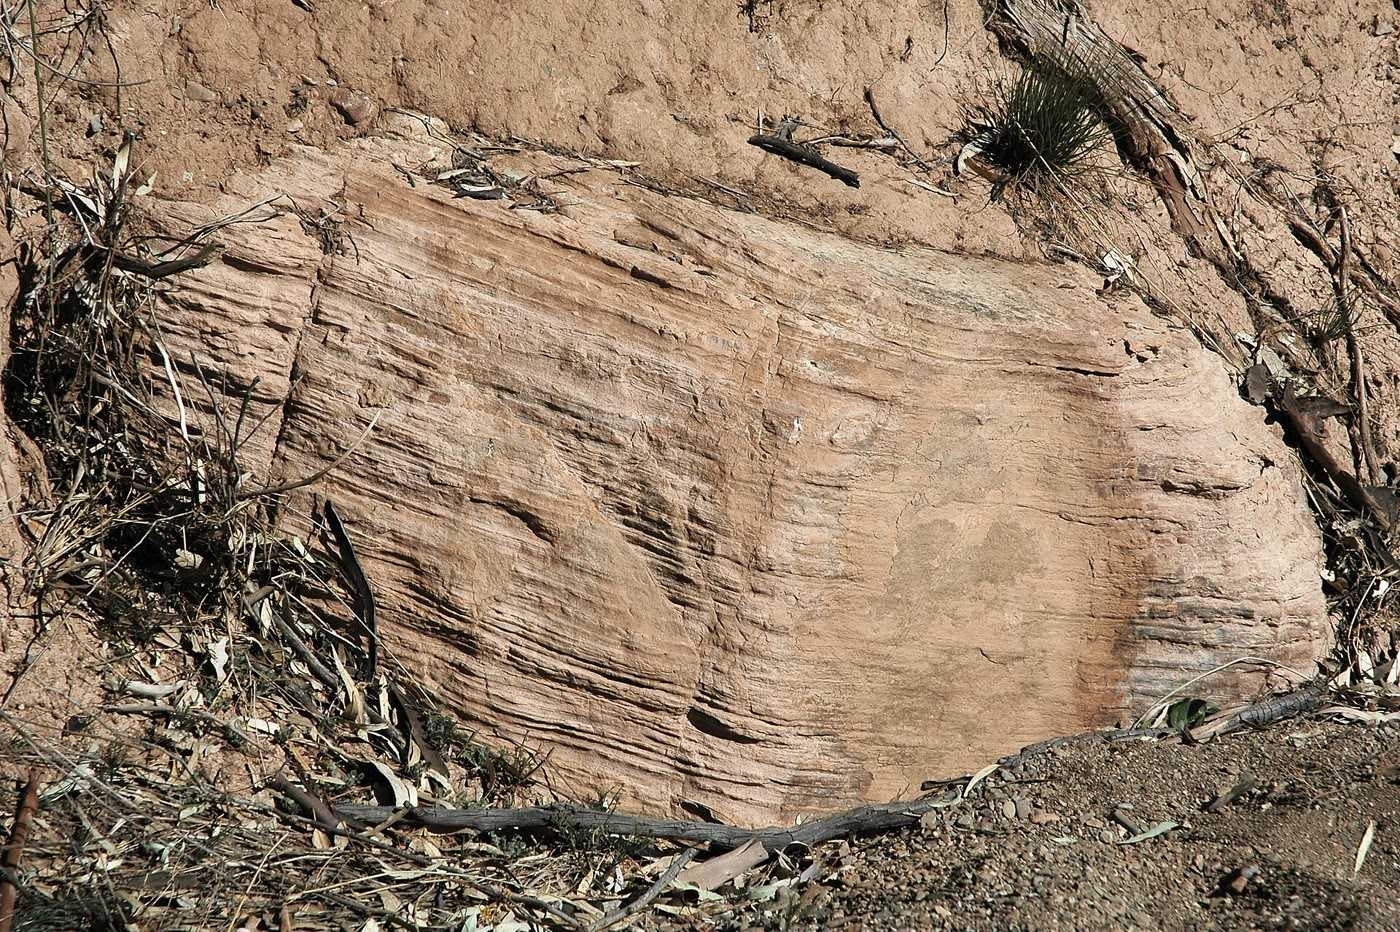
\includegraphics[width=0.66\linewidth]{images/book4/b2-18-cap-carbonate.jpg}
\par\smallskip{\small \omterm{def:b2:precambrian-earth:snowball}{盖帽碳酸盐岩}：Nuccaleena 组的层状白云岩，
位于南澳大利亚弗林德斯山脉，覆于马里诺冰期的沉积之上
（岩层倾斜）。照片：James St.~John, CC~BY~2.0（维基共享资源）。}
\end{omfigure}

成冰纪的两次雪球事件现已由火山灰中锆石的铀–铅年龄定年，
并由富含有机质页岩的铼–锇年龄定年。斯图特冰期始于 717.5 至 \qty{716.3}{Ma} 之间，
结束于 659.3 至 \qty{658.5}{Ma} 之间，持续 \qty{58}{Ma}，起止时间在全球范围内同步。
马里诺冰期始于 649.9 至
\qty{639.0}{Ma} 之间，年代约略测定。结束于 636.0 至 \qty{634.7}{Ma} 之间，
持续至少 \qty{3}{Ma}。每次冰期都以单一的\omterm{def:b2:precambrian-earth:snowball}{盖帽碳酸盐岩}结束，从不出现多层。铁建造
中断 10 亿年后，又重新出现于斯图特冰期的沉积中。
至少还有一次更早的雪球事件，发生于成铁纪约 \qty{2.4}{Ga}，恰逢\omterm{def:b2:precambrian-earth:goe}{大氧化事件}（GOE）；
两次事件之间约 \qty{1.5}{Ga} 的时间里，几乎没有已知的冰盖。
% ledger: hoffman17:ages, hoffman17:cryochrons, hoffman17:cap, hoffman17:models, hoffman17:earlier

\begin{history}[从古怪的假说到有定年依据的理论]
1964 年，W.~B. 哈兰德注意到晚前寒武纪冰川作用的证据。
1968 和 1969 年，M.~I. 布德科以及用类似模型工作的 W.~D. 塞勒斯发现，
\omterm{def:b2:precambrian-earth:ice-albedo}{冰–反照率反馈}可使冰层在推进足够远后扩展至赤道；一个全球冻结的地球
被视为一种不可逆的状态，因而被认为从未发生过。
1981 年，J.~沃克、P.~海斯与 J.~卡斯廷描述了硅酸盐风化恒温器，
并指出，在冻结的地球上，火山释放的二氧化碳会不断积累，直至冰层融化：
这一状态可以自行结束。1992 年，J.~L. 基尔施文克提出它实际上曾经发生过，
并将其命名为“\omterm{def:b2:precambrian-earth:snowball}{雪球地球}”；1998 年，P.~F. 霍夫曼等人发表了
“A Neoproterozoic Snowball Earth”一文，全冰川期此后被称为“冰冻期”（cryochron）。
2004 年以前，尚无成冰纪冰川沉积经放射性测年。
上文所列年代，是此后数年研究的成果。
\end{history}
% ledger: hoffman17:history

火山是出路。在覆冰的地球上，降雨与河流几乎停止，硅酸盐风化随之
停止，火山释放的二氧化碳便在大气中积累，
直到其温室效应使冰层融化。

\begin{proposition}[二氧化碳的积累]\label{prop:b2:precambrian-earth:co2}
设二氧化碳以速率 $F$（每年的质量）释放到质量为
$M_{\text{a}}$、平均摩尔质量为 $\bar M$ 的大气中，且无汇，则使其体积
混合比由近零升至 $x$ 所需的时间为
\[
  \tau = \frac{x}{1 - x}\,\frac{M_{\mathrm{CO_2}}}{\bar M}\,\frac{M_{\text{a}}}{F} .
\]
\end{proposition}

\begin{proof}
大气中含其他气体 $n = M_{\text{a}}/\bar M$ 摩尔。加入 $n_c$ 摩尔
二氧化碳后，其混合比为 $x = n_c/(n + n_c)$，因此 $n_c = n\,x/(1 - x)$，其质量为
$n_c M_{\mathrm{CO_2}}$，以速率 $F$ 释放所需时间为 $\tau = n_c M_{\mathrm{CO_2}}/F$。
\end{proof}

\begin{example}[脱离雪球状态需要多久？]\label{ex:b2:precambrian-earth:escape}
今日火山释放量的最高优选估计值为每年 \qty{0.26}{Gt} 的
二氧化碳。结束成冰纪雪球所需的
混合比估计值介于 0.01 至 0.1 之间。取 $M_{\text{a}} =
\qty{5.1e18}{kg}$，$\bar M = \qty{28.97}{g.mol^{-1}}$ 与 $M_{\mathrm{CO_2}} =
\qty{44.01}{g.mol^{-1}}$，$x = 0.01$ 所需时间为 $\frac{0.01}{0.99}\times1.519\times\qty{5.1e18}{kg}
/ \qty{0.26e12}{kg.\text{年}^{-1}} = \qty{0.30}{Ma}$，而 $x = 0.1$ 需 \qty{3.3}{Ma}。
\end{example}
% ledger: usgs:volcanic-co2, hoffman17:co2, earth:Matm, earth:Mmol, ciaaw:abridged-2024
% values: co2_t001_Myr 0.301, co2_t01_Myr 3.311 (precambrian.py)

覆盖全球、压强为 \qty{1}{bar} 的纯二氧化碳柱，若以同样速率累积，需要
\qty{20}{Ma}，这是沃克、海斯与卡斯廷给出的数值。几百万年
已经很长，但斯图特冰期持续了 \qty{58}{Ma}。要么是阈值更高，
或是脱气量更低，或冻结的地球仍有汇：年轻海底的风化，
在冰下也不停止，是一种可能的汇。在能量平衡模型中，脱离
雪球状态需要有效发射率下降，直到温度达到 \qty{263}{K}，
在成冰纪太阳（今日的 \qty{94}{\percent}）照射下，有效发射率由 0.616 降至 0.472，
额外截留约 \qty{39}{W.m^{-2}}（见\cref{exo:b2:precambrian-earth:10}）。
% ledger: hoffman17:co2, hoffman17:models, usgs:volcanic-co2
% values: one_bar_Myr 19.98, eps_melt_094 0.4716, forcing_melt_094 39.1 (precambrian.py)

当冰层终于在赤道处裂开时，反馈反向运行：暗色海洋吸收了更多
阳光，冰层退缩，模型中冰线约在
\qty{2}{ka} 内迅速退向两极。地球随即处于暗色地表上的巨大温室效应之中，一场炎热的
余波。风化在那种气候下极为迅速，将钙、镁与碳酸氢盐倾入
海洋之中，\omterm{def:b2:precambrian-earth:snowball}{盖帽碳酸盐岩}在此沉淀，同时融水淹没陆架；此后需要
约一千万年，才能使二氧化碳重新降下来。冰盖与\omterm{def:b2:precambrian-earth:snowball}{盖帽碳酸盐岩}、
\omterm{def:b2:precambrian-earth:bif}{条带状铁建造}与同步年龄，是如今多数地质学家接受成冰纪雪球事件确已发生的依据，
尽管其严酷程度如何——赤道是否残存一条开阔水带，如“水带”模型所提出的——
仍存争议。
% ledger: hoffman17:hysteresis, hoffman17:cap, hoffman17:debate

\section*{练习}\label{sec:b2:precambrian-earth:exercises}

除另有说明外，练习所用数据如下：$\sigma = \qty{5.670e-8}{W.m^{-2}.K^{-4}}$；
$S_0 = \qty{1361}{W.m^{-2}}$；今日反照率为 0.294，地表平均温度为 \qty{288}{K}；
雪球反照率为 0.6；过渡段从 \qty{263}{K} 到 \qty{283}{K}；今日有效发射率
为 0.616；古夫定律 $L/L_0 = 1/(1 + 0.4\,t/t_\odot)$ 适用于距今 $t$ 时刻，$t_\odot =
\qty{4.567}{Ga}$；\omterm{def:b2:precambrian-earth:greenstone}{科马提岩}液相线在 MgO 为 \qty{32.2}{\percent} 时为 \qty{1616}{\celsius}，
斜率为每百分点 \qty{18.0}{\celsius}；半衰期分别为 \ce{^{238}U} \qty{4.468}{Ga}，\ce{^{235}U}
\qty{0.704}{Ga}, \ce{^{232}Th} \qty{14.0}{Ga}, \ce{^{40}K} \qty{1.248}{Ga}.
% ledger: const:sigma, earth:TSI, earth:albedo, earth:Tsurf, hoffman17:models, gough81:luminosity, connelly12:cai, so16:liquidus, iaea:isotopes

\begin{exercise}[$\star$]\label{exo:b2:precambrian-earth:1}
（a）\omterm{def:b2:precambrian-earth:eons}{冥古宙}、\omterm{def:b2:precambrian-earth:eons}{太古宙}与\omterm{def:b2:precambrian-earth:eons}{元古宙}各持续了多久？（b）三者合计占地球年龄的
几分之几？（c）已知最古老锆石结晶时，地球
已有多大年龄，最古老岩石形成时又是多大年龄？
\end{exercise}

\begin{exercise}[$\star$]\label{exo:b2:precambrian-earth:2}
今日\omterm{def:b2:elements-in-the-earth:bse}{全硅酸盐地球}每千克释放的热量中，\ce{^{238}U} 占 \qty{1.917}{pW}，
\qty{0.082}{pW} 来自 \ce{^{235}U}，\qty{2.089}{pW} 来自 \ce{^{232}Th}，以及 \qty{0.818}{pW} 来自
\ce{^{40}K}（$\qty{1}{pW} = \qty{e-12}{W}$）。（a）求各项在 \qty{3}{Ga} 前的贡献及
总和。（b）产热率自那时以来降低了多少倍？（c）今日哪种同位素
占主导，当时又是哪一种？
\end{exercise}

\begin{exercise}[$\star$]\label{exo:b2:precambrian-earth:3}
利用\omterm{def:b2:precambrian-earth:greenstone}{科马提岩}温度计。（a）求含
\qty{28}{\percent} MgO 的\omterm{def:b2:precambrian-earth:greenstone}{科马提岩}，其液相线是多少？（b）\qty{1500}{\celsius} 对应的 MgO 含量是多少？（c）一
具鬣刺结构的熔岩流，全岩 MgO 为 \qty{38}{\percent}。为何其液相线不应
直接从该直线上读取？
\end{exercise}

\begin{exercise}[$\star$]\label{exo:b2:precambrian-earth:4}
将下列事件按时间先后排列，并给出大致年龄：\omterm{def:b2:precambrian-earth:goe}{大氧化事件}、
最早的叠层石、马林诺冰期的结束、常见\omterm{def:b2:precambrian-earth:greenstone}{科马提岩}的最后出现、
最古老的岩石、氧气的第二次上升、最早的埃迪卡拉纪化石、
皮尔巴拉穹隆–龙骨构造的结束。
\end{exercise}

\begin{exercise}[$\star\star$]\label{exo:b2:precambrian-earth:5}
（a）验证今日地球的有效发射率为 0.616。（b）求今日太阳照射下
雪球的平衡。（c）证明中间平衡 \qty{275.5}{K} 满足
$R = E$，误差在 \qty{0.5}{W.m^{-2}} 之内。（d）求此处 $R$ 与 $E$ 的
斜率，并断定该平衡不稳定。
\end{exercise}

\begin{exercise}[$\star\star$]\label{exo:b2:precambrian-earth:6}
（a）利用古夫定律，求 \qty{2.4}{Ga} 前与 \qty{0.65}{Ga} 前的日照量，分别
占今日的几分之几。（b）在模型中，取今日的发射率，各时刻是否都可能出现暖气候？
（c）霍夫曼等人指出，成铁纪太阳比成冰纪太阳约暗 \qty{10}{\percent}，
请核验这一说法。
\end{exercise}

\begin{exercise}[$\star\star$]\label{exo:b2:precambrian-earth:7}
斯图特冰期自 \qty{716.9}{Ma} 延续至 \qty{658.9}{Ma}（取定年区间的中点），
马林诺冰期自 \qty{644.5}{Ma} 至 \qty{635.4}{Ma}。（a）求二者的时长及
两者之间的间冰期。（b）按这些数据，成冰纪（720 至 \qty{635}{Ma}）
期间，冰盖覆盖地球的时间占多少比例？（c）为何马林诺冰期的时长只是一个
粗略的数值？
\end{exercise}

\begin{exercise}[$\star\star$]\label{exo:b2:precambrian-earth:8}
（a）火山以每年 \qty{0.26}{Gt} 的速率释放且无汇，使空气中二氧化碳
混合比达到 0.05 需要多长时间？（b）这是 1750 年 \qty{278}{ppm} 的多少倍？（c）若释放量的一半被海底风化吸收，
则需要多长时间？
\end{exercise}
% ledger: usgs:volcanic-co2, earth:Matm, earth:Mmol, ciaaw:abridged-2024, ipcc:erf-2xco2

\begin{exercise}[$\star\star$]\label{exo:b2:precambrian-earth:9}
一套新元古代杂砾岩含有擦痕砾石，其中一些位于细纹层理的泥中，
这些泥层在砾石下方向下弯曲。（a）这一弯曲说明了什么？（b）其古纬度为
\ang{10}。这对雪球假说有何意义？（c）其上直接覆盖着一层
厚几米的粉红色纹层状白云岩。它是什么？它记录了什么？
\end{exercise}

\begin{exercise}[$\star\star\star$]\label{exo:b2:precambrian-earth:10}
在成冰纪太阳下，$S = 0.94\,S_0$。（a）证明在该模型中暖态仍
勉强存在，但雪球态也存在。（b）求雪球在
今日发射率下的温度。（c）求雪球升至 \qty{263}{K} 并融化时的
发射率。（d）将发射率的变化换算为
\qty{263}{K} 时额外截留的长波辐射，单位为 \unit{W.m^{-2}}。
\end{exercise}

\begin{exercise}[$\star\star\star$]\label{exo:b2:precambrian-earth:11}
（a）利用\cref{prop:b2:precambrian-earth:tipping}中的临界点，证明磁滞回线
的宽度 $S_{\text{m}}/S_{\text{f}}$ 与发射率无关，并
求出其值。（b）什么会使回线变窄？（c）为何雪球只能在远离
其冻结时的条件下融化？
\end{exercise}

\begin{exercise}[$\star\star\star$]\label{exo:b2:precambrian-earth:12}
推导暖平衡态附近能量平衡模型的时间常数 $\tau =
C/(E'(T^*) - R'(T^*))$，并对深度为 \qty{50}{m}、密度为
\qty{1025}{kg.m^{-3}}、比热容为 \qty{3992}{J.kg^{-1}.K^{-1}} 的海洋混合层求其值。当日射量
趋近左侧临界点时，$\tau$ 在本模型中将如何变化，
以及在反照率随温度平滑变化的模型中将如何变化？
\end{exercise}
% ledger: noaa:seawater-1025, teos10:cp0

\begin{problem}[{周末问题——更炽热的年轻地球}]\label{pb:b2:precambrian-earth:1}
本题追踪年轻地球从内部到大气的演化，请利用
各练习的数据。按质量计，\omterm{def:b2:elements-in-the-earth:bse}{全硅酸盐地球}含铀 \qty{0.0203}{ppm}、钍 \qty{0.0795}{ppm}、
钾 \qty{240}{ppm}；其同位素每千克释放的功率分别为 \qty{95.13}{\micro W}
（\ce{^{238}U}）、\qty{568.47}{\micro W}（\ce{^{235}U}）、\qty{26.28}{\micro W}（\ce{^{232}Th}）及
\qty{28.47}{\micro W}（\ce{^{40}K}）。按质量计，铀中
\qty{99.29}{\percent} 为 \ce{^{238}U}、\qty{0.711}{\percent} 为 \ce{^{235}U}，钾中
\qty{0.0120}{\percent} 为 \ce{^{40}K}。结果保留三位有效数字。

\noindent\textbf{第一部分——来自内部的热量。}
\begin{enumerate}
  \item 求今日每种同位素在每千克\omterm{def:b2:elements-in-the-earth:bse}{全硅酸盐地球}中释放的热量，单位为
        \unit{pW.kg^{-1}}。
  \item 求总热量。
  \item 求每种同位素的衰变常数，单位为 \unit{Ga^{-1}}。
  \item 求派克丘\omterm{def:b2:precambrian-earth:greenstone}{科马提岩}于 \qty{2.7}{Ga} 前喷发时各项的贡献。
  \item 求当时的总热量，以及其与今日总热量之比。
  \item 当时哪种同位素释放的热量最多？为何它今日释放的热量如此之少？
\end{enumerate}

\noindent\textbf{第二部分——\omterm{def:b2:precambrian-earth:eons}{太古宙}的太阳。}
\begin{enumerate}[resume]
  \item 利用高夫定律，求 \qty{2.7}{Ga} 前的日射量占今日的比例，并
        以 \unit{W.m^{-2}} 为单位给出其值。
  \item 取今日发射率，求该日射量下的暖平衡态，它是否
        为该模型中有效的暖态？
  \item 求该日射量下的雪球平衡态。
  \item 在暖态反照率下，要使地球保持在 \qty{288}{K}，有效发射率应为多少？
  \item 仅靠二氧化碳即可达到这一效果：\qty{2.5}{Ga} 时其分压为 0.004 至 \qty{0.03}{bar}。
        若大气压约为 \qty{1}{bar}，则该值是 1750 年
        \qty{278}{ppm} 的多少倍？
  \item 指出使二氧化碳长达数亿年维持在此水平的
        过程名称。
\end{enumerate}

\noindent\textbf{第三部分——雪球及其终结。}
\begin{enumerate}[resume]
  \item 第一次雪球事件发生于 \qty{2.4}{Ga} 前：求当时的日射量占今日的比例。
        取今日发射率，该模型的暖态是否仍然可能？
  \item 二氧化碳以每年 \qty{0.26}{Gt} 的速率输入，混合比
        达到 0.1 需要多长时间？
  \item 若在较暗的成铁纪太阳之下阈值高出一倍、即为 0.2，则需要多长时间？
  \item 哪种岩石记录了雪球的终结？它是如何记录的？
  \item 为何斯图尔特冰期的铁建造需要冰下缺氧的海洋？
\end{enumerate}

\noindent\textbf{第四部分——\omterm{def:b2:precambrian-earth:greenstone}{科马提岩}温度计。}
\begin{enumerate}[resume]
  \item 由两组实验检验\omterm{def:b2:precambrian-earth:greenstone}{科马提岩}线的斜率。
  \item 派克丘的一种\omterm{def:b2:precambrian-earth:greenstone}{科马提岩}熔体含 \qty{30}{\percent} MgO，求其液相线温度。
  \item 求巴伯顿\omterm{def:b2:precambrian-earth:greenstone}{科马提岩}的液相线温度，其 MgO 含量为 \qty{32.2}{\percent}。
  \item 求 MgO 含量为 \qty{12}{\percent} 的原生洋脊玄武岩的液相线温度。
  \item 若改用基拉韦厄斜率，即每个百分点 \qty{20}{\celsius}，
        则从巴伯顿点出发，玄武岩的温度将是多少？斜率的选择影响有多大？
  \item 为何两种熔岩之间的温差
        大于\omterm{def:b2:precambrian-earth:eons}{太古宙}与今日地幔的位温之差？
  \item 综合来看：\omterm{def:b2:precambrian-earth:eons}{太古宙}最热的\omterm{def:b2:precambrian-earth:greenstone}{科马提岩}熔岩比今日洋脊原生玄武岩
        高出多少度？
\end{enumerate}
\end{problem}
% ledger: ms95:pm-trace, dye:isotope-heat, iaea:isotopes, gough81:luminosity, cz20:archean-air, ipcc:erf-2xco2, usgs:volcanic-co2, hoffman17:co2, so16:liquidus, helz98:glass-thermometer, pierru22:komatiite
